\section{Enter missing values/overview}Here you can see an overview of all clients that will be created. Please enter missing values and correct false values.\\
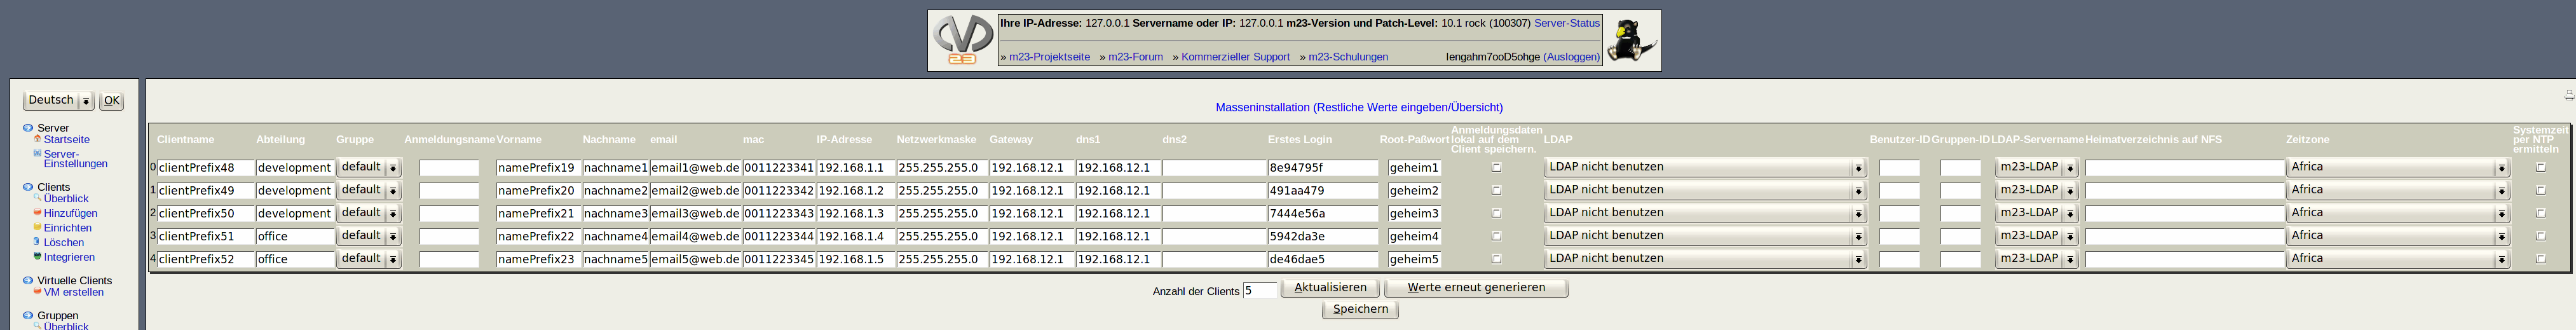
\includegraphics[scale=0.33]{/mdk/doc/manual/screenshots/en/mi_step4.png} \\
\subsection{Change the number of clients}
You can change the number of clients by entering a new value in the field \textit{"Number of clients"}. Click on \textit{"Refresh"} if you want to lower the amount or on \textit{"Regenerate values"} to increase.\\
\textit{"Regenerate values"} can generate new values or read additional lines from the database file, whereas \textit{"Refresh"} can only delete clients. If there are not enough lines in the database file, these values have to be entered by hand. The generation of a huge amount of values can take a long time. E.g. "pinging" of clients.\\
To start the installation click on \textit{"Save"}.\\
